Feed-forward networks can theoretically be used for image recognition. However, there are several issues with this. Firstly, even very low resolution 32x32 pixel garyscale images require some 1024 inputs (for each pixel) each connected to each of the $k$ neurons in the next layer, giving $1024k$ parameters to train in the first layer alone. Since it receives the pixels as a 1024-dimension vector, the network has no spatial awareness. For example it has no intrinsic knowledge that pixel numbers 1, 2, 33 and 34 form a square, and that it is above (and thus related to) the square formed by pixels 65,66,97 and 98. To learn this, we would need a very good dataset, long training times and a rather deep network. The requirements mean that a network need to be exceedingly complex, and thus computationally expensive to train to a good accuracy.

\begin{figure}[h!]
\centering
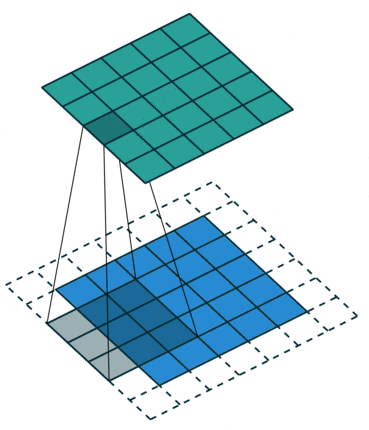
\includegraphics[scale=0.45]{pictures/conv}
\caption{Image showing a convolution operation, where the input is in blue, the ouput is in cyan and the weight matrix is the shaded region \cite{convPics}.}
\label{fig:conv}
\end{figure}

Convolutional neural networks tackle all these issues. The network architecture is now made up of several convolutional layers, followed by several feed forward layers. Convolutional operations are  spatial operations, meaning that spatial knowledge is directly encoded into the operation of the neural network. Convolutional layers are able to extract spatial features from the image, which the feedforward layer can then use to classify the image. For a 2D image, an $n \times n$ weight matrix $W_{i,j}$ (also called the kernel or filter) where $n$ is odd goes over the image in a certain stride (another hyperparameter), applying a convolution operation. There may be multiple weight matrices in a single layer, and the result of these operations then forms the input of the next layer, which may also be a convolution. The convolution operation can be thought of as the mathematical equivalent of pattern matching. The equation for a convolution operation on  the 2D matrix $x_{i,j}$ is
\begin{equation}
y_{i,j} = \sum^{\frac{n-1}{2}}_{k=-\frac{n-1}{2}} \sum^{\frac{n-1}{2}}_{l=-\frac{n-1}{2}} W_{k,l} x_{i+k,j+l} 
\end{equation}
thus each value in the weight matrix is multiplied with the corresponding pixel in the $n \times n$ region about pixel i,j (see figure \ref{fig:conv}). The size of $n \times n$ then defines a "receptive field", essentially a size of feature that can be extracted. The layer will also have a stride parameter, describing how much $i$ or $j$ should increase by with successive convolutional operations. 


Convolutional neural networks not only introduce spatial relationships via the convolution operation, but also drastically reduce complexity, since only $n \times n \times m = mn^2$ parameters need training per convolutional layer, with $m$ the number of weight matrices per layer. Common values for the first layer are $n=3$, $m=16$, which gives 144 learnable parameters in the first layer, far less than the $1024k$ in the feed forward case. The fact that each individual layer is cheaper means that the network can be made much deeper. Pooling layers are often placed in between convolutional layers. Pooling reduces the size of the image, allowing the next convolutional layer to extract features which are in effect larger in the original picture (given that the weight matrix is the same size), allowing progressively larger features to be built up from smaller ones. Once several layers of convolution and pooling have extracted the spatial features, the final feed forward layer uses these to classify like a regular neural network.  

The extension of CNNs to 3D space is trivial, the original inputs and thus the weight matrices are simply extended to 3D matrices.